% File example.tex
% Contact: simonnet@ecole.ensicaen.fr
%
% version 1.0 (July 24, 2009)
% version 1.1 (September 3, 2009)
% add using of the optional command: \secondauthoraddr

\documentclass[10pt]{article}

% File icdp2009.sty
% Preamble that you have to include to use the template  

% July 24, 2009
% Contact: simonnet@ecole.ensicaen.fr


\usepackage[a4paper,textwidth=18cm,textheight=24cm,top=2.85cm, bottom=2.85cm, left=1.5cm, right=1.5cm]{geometry}

\usepackage{includes/icdp2009}

% left justified caption
\makeatletter
\long\def\@makecaption#1#2{%
\vskip\abovecaptionskip
\sbox\@tempboxa{#1. #2}%
\ifdim \wd\@tempboxa >\hsize
#1. #2\par
\else
\global \@minipagefalse
\hb@xt@\hsize{\box\@tempboxa\hfil}%
\fi
\vskip\belowcaptionskip}
\makeatother




%other package

% vectorial font
%\usepackage{lmodern}

\usepackage{graphicx}
\usepackage{times}

\usepackage{textcomp}
\usepackage[justification=centering]{caption}
\usepackage{subcaption}
\usepackage{enumitem}
\usepackage[caption=false]{subfig}
\usepackage{enumitem}
\usepackage{multirow}

\begin{document}
\noindent

% This should produce references in the order they appear
\bibliographystyle{ieeetr}

%\title{Automatically landmarks prediction on Beetle's pronotum}
%\title{Deep network for landmarks prediction on Beetle pronotums}
%\title{Two scenarios to predict landmarks on Beetle pronotum by Deep Network}
\title{Towards landmarks prediction with Deep Network}

\authorname{Van Linh Le$^{1,3}$, Marie Beurton-Aimar$^{1}$, Akka Zemmari$^1$, Nicolas Parisey$^2$}
\authoraddr{$^1$LaBRI - CNRS 5800 Bordeaux University, France, van-linh.le/beurton/zemmari@labri.fr}

%optional
\secondauthoraddr{$^2$IGEPP - INRA 1349, France, nparisey@rennes.inra.fr }
\thirdauthoraddr{$^3$ITDLU - Dalat University, Vietnam, linhlv@dlu.edu.vn}


\maketitle

\keywords
Landmarks, convolutional neural networks, fine-tuning, recogntion, procrustes.

\abstract
Morphometry landmarks are used in many biological
applications. Mostly, the landmarks are defined manually or
semi-automatic by applying the image processing techniques. In recent
years, deep learning is known as a good solution for the difficult
problems in computer vision. It appears in many fields such as
classification, recognition, face detection. In the context applying
deep learning to solve the regression problems, in this paper, we
present a convolutional neural network to predict the landmarks on 2D
images, specify beetle's images. The experiments on the
proposed network have been done in two ways: training from scratch and
fine-tuning from a trained model. The dataset includes the images of 
collecting from $253$ beetles. For each beetle, the images of 5 parts 
have been extracted(\textit{head, pronotum, body, left and right mandible}).
 Among these, a set of manual landmarks has been built for each part by 
the biologists. In this task, we use the images of 3 parts (head, pronotum, and body) with the main purpose to predict the landmarks on pronotum images.
 The quality of predicted landmarks
is evaluated by calculating the distance in pixels between the
coordinates of the predicted landmarks and manual landmarks which are
considered as ground truth.


\section{Introduction}
Morphometrics landmarks (or point of interest) is important features
in many biological investigations. They are  usually used to analyze
the forms of biological organs or organisms. Their analysis is mainly
based on their coordinates. Depending on the problem to study, the number of
landmarks may be more or less high and  their location  can
be on the shape (border) or inside the object. For
  examples, the landmarks on Drosophila wings \cite{drosophilaWings} have stayed on the
veins of the wings but the landmarks on human ear \cite{cintas2016automatic} can be located at
the ear border or inside it. Currently, the landmarks are set manually by
the biologists, one can note that this work is time-consuming and difficult to
reproduce, therefore, a method that proposes automatically the
coordinates of landmarks could be a concern.

In image processing, segmentation is most often the first and the most
important step. This task remains a bootleneck to compute features of
an image. In some cases, the object of interest is easy to extract and
can be analyze with the help of a lot of very well-known image
analysis procedures. In a previous studying \cite{le2017maelab}, we have analyzed beetle
mandibules with a set of algorithms based on the Hough Transform
procedure \cite{palaniswamy2010automatic}, SIFT
\cite{lowe2004distinctive} and SURF \cite{bay2006surf} algorithms could also be
suitable to work on this topic for example. But in some cases, the question of how to segment the
object of interest consumes the most part of a time project. It is why
we have turned our studying to a way to analyze image without a
segmentation step. The application has been again on beetles images
but on \textit{pronotum, head, body} parts. As these parts have not
been separated from each other, their segmentation by image processing
procedures has been given up. Coordinates of manual landmarks for each part
have been provided and are considered as the ground
truth to evaluated the predicted landmarks by the algorithms. We have focus on the
pronotum parts for this studying, see (Fig.\ref{figpronotum}) to see
the $8$ landmarks that we are looking for.


To achieve the landmarks prediction, a Convolutional Neural Network
(CNN)\cite{lecun2010convolutional} has been designed based on Lasagne
library\cite{lasagne}. From a first model version, the network has been
trained from scratch on the dataset of pronotum images. In a second
step the training has been modified to include a fine-tuning
\cite{yosinski2014transferable} stage.



\begin{figure}[htbp]
\centering
	\centerline{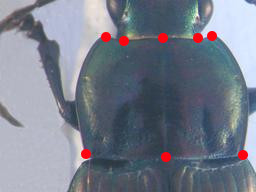
\includegraphics[scale=0.7]{images/pronotum}}
	\caption{\small{An example of pronotum images and its manual landmarks}}
	\label{figpronotum}
\end{figure}

In the next section, we present related works about automatic
estimation landmarks on 2D images. In section $3$, we present the
architecture of the network and the procedure to enlarge the data
set. In section $4$ we compare the results obtained with the first
model and these ones after fine-tuning. 


\section{Related works}
Deep learning methods are coming from machine learning theory. They
have been introduced in the middle of previous century for artificial
intelligence applications but their application encounters problems to
take into account real cases. More recently, the improvement of computing capacities, both in
memory size and time with GPU programming has opened a new challenge  
for deep learning. Many deep learning architectures have been proposed
to solve the problems of classification \cite{krizhevsky2012imagenet,
  ciregan2012multi}, image recognition \cite{szegedy2015going,
  farabet2013learning, li2015convolutional}, speech recognition
\cite{mikolov2011strategies, hinton2012deep} and language translation
\cite{jean2014using, sutskever2014sequence}. Along with that
developments, many frameworks have been built such as Caffe
\cite{jia2014caffe}, Theano \cite{2016arXiv160502688short}, Tensorflow
\cite{tensorflow2015},.... These frameworks help
the users to design their application by re-using networks
architecture they propose. In image analysis domain,
deep learning, specifically with CNN, can be used to predict the key points on
the image. Yi Sun et al. \cite{sun2013deep} have proposed a cascaded
convolutional network to predict the key points on the human
face. Zhang et al. \cite{zhang2014facial} optimizes facial landmarks
detection with a set of related tasks such as head pose estimation,
age estimation, .... Cintas et al. \cite{cintas2016automatic} have
introduced a network to predict the landmarks on human ear images to
characterize ear shape.


In geometric morphometry, landmarks or points of interest are one of
the important features. Landmark studies have traditionally
analyzed on 2D images. Depending on if the analyzed images are
easy or not to segment, setting landmarks can apply
the different methods. When segmentation can be applied, Lowe et
al. \cite{lowe2004distinctive} have proposed a method to identify the
key points in the 2D image. From the detected key points, the method
is able to match two images. Palaniswamy et
al. \cite{palaniswamy2010automatic} have applied probabilistic Hough
Transform to automatically estimate the landmarks in images of
Drosophila wings. Krahenbuhl et al. \cite{le2017maelab} have extended
Palaniswamy's method to detect landmarks automatically on beetles
mandibles. Unfortunately, after testing, when the segmentation has not good quality,
we have observed that re-using this method produces too many
noises. This is why we have turned our work on deep learning
algorithms in order to find suitable solution to predict the landmarks
on images hard to segment.


\section{Network model}
Deep learning is a learning method with multiple levels of
representation of connected layers (convolutional neural
network). Data representation is transformed from a lower level to a
higher one with many complex functions that can be learned via
backpropagation. In this section, we present the initial version of the CNN that we have used
to begin to predict the landmarks. 

\subsection{Network architecture}
\label{secmodel}
The first step to work in CNN is to study the network
architecture. After several tests, we have chosen to work with a model provided in Lasagne framework \cite{lasagne} coming from
Theano \cite{2016arXiv160502688short}. We will first present the
original model and then, we will describe how we have modified it by definition of an
\textit{elementary block} that we compose in the final model.

Like the networks have been proposed by LeCun et al. \cite{lecun2010convolutional}, Li et al. \cite{li2015convolutional}, and Cintas et al. \cite{cintas2016automatic}, the proposed network consists of common layers
with different learnable parameters. It receives an input image with
the size  $1 \times 256 \times 192$ to train, to validate, and to
test. The network consists of three repeated-structures of a convolutional layer
followed by a pooling layer (keeping the maximum value). The depth of convolutional layers increases with different size of the filter kernels.
All the kernels of pooling layers have the same size. 
At the end, three full connected layers are added to the
network. The output of the last full-connected
layer corresponds to the $16$ values which are the coordinates of the
$8$ landmarks to predict.


Experiments with this origin model show that this architecture is still
not good enough to predict the landmark positions precisely. For
instance, overfitting appears during training and validation
steps. Srivastava et al. \cite{srivastava2014dropout} suggest to use
dropout sequence to correct overfitting artefacts. Dropout step randomly drops units from the
neural network during training and so includes some variations between
the different runs. We have updated the model architecture in that
way. An \textit{elementary block} is defined as a sequence of
convolution (\textit{$C_i$}), pooling (\textit{$P_i$}) and dropout(\textit{$D_i$}) layers that can be repeated several
times before to achieve the computation with the full-connected
layers. For our purpose, we have assembled $3$ \textit{elementary
  blocks} in our model (see Fig.\ref{cnnnetwork2}). The parameters for
each layer are as below, the list of values follows the order of
\textit{elementary blocks} :

\begin{itemize}[nosep,label=\footnotesize$\bullet$]

\item CONV layers:
		\begin{itemize}[nosep]
			\item Number of filters: $32, 64,$ and $128$,
			\item Kernel filters size: $(3 \times 3), (2 \times 2),$ and $(2 \times 2)$,
			\item Stride values: $1, 1, 1$,
			\item No padding is used for CONV layers.
		\end{itemize}			
	\item POOL layers:
		\begin{itemize}[nosep]
			\item Kernel filters size: $(2 \times 2), (2 \times 2),$ and $(2 \times 2)$,
			\item Stride values: $2, 2, 2$.
			\item No padding is used for POOL layers.
		\end{itemize}
	\item DROP layers: 
		\begin{itemize}[nosep]
			\item Propabilities: $0.1, 0.2, $ and $0.3$.
		\end{itemize}
	\end{itemize}
In the last fool connected layers (FC), the parameters are : FC1 output :
$1000$, FC2 output : $1000$, FC3  output : $16$. As usual, a dropout layer is
inserted between FC1 ond FC2 with a probability equal to $0.5$.


\begin{figure*}[!t]
\centering
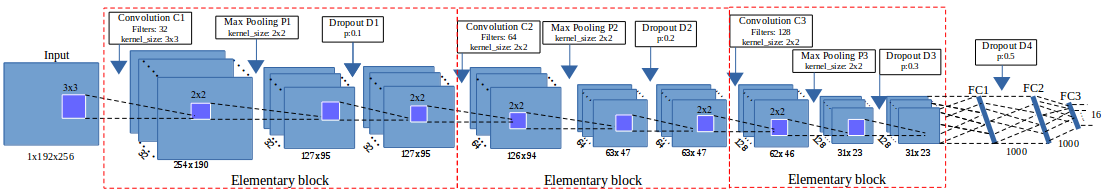
\includegraphics[scale=0.32]{images/arch_model}
\caption{{\small{Network architecture using $3$ \textit{elementary blocks}.
  Convolution
  layer in red, pooling in yellow and dropout in green color.}}} 
\label{cnnnetwork2}
\end{figure*}

During training, the values of learnable parameters have been updated
to increase the accuracy of the network by applying gradient descent
in backward phase. Therefore, the network is designed with a small
sharing learning rate and momentum. Their values are updated over
training time to fit with the number of epochs\footnote{An epoch is a
  single pass through the full training set.}. The network is designed
to finish the training in $5000$ epochs. The learning rate was
initialized at $0.03$ and stopped at $0.00001$, while the momentum was
updated from $0.9$ to $0.9999$.


The implementation of the network is done
on Lasagne framework \cite{lasagne} which allows computing on GPU. The
network has been trained on NVIDIA TITAN X cards.


\subsection{Expanding the data set}
\label{sec_data}
The data set includes $293$ images of beetles (for each part). All
images are taken with the same camera in the same condition with a
resolution of $3264 \times 2448$. Each image has $8$ manual
landmarks setting by biologists (Fig. \ref{figpronotum}). Thte
experiments have been designed with a testing set which  includes $33$
and the remained $260$ images are put in two equal subsets one for
training and one for validation. For performance considerations, in most of CNNs
\cite{lecun2010convolutional, sun2013deep,  krizhevsky2012imagenet,
  cintas2016automatic}, the size of the input is limited to $256
\times 256$ pixels, thus we have down-sampling our images to a new
resolution $256 \times 192$ (to respect the ratio between $x$ and
$y$), of course the coordinates of manual landmarks have been also
scaled to fit with the new resolution.


One of the main characteristics of CNN is to deal with a huge size of
dataset and one can consider that only several hundreds of images is
not relevent to use CNN. Moreover, working with small dataset can push
us again to the popular problem of \textit{overfitting}. A way to  to
enlarge the dataset size has to be considered. In image processing, we usually apply
transform procedures (translation, rotation) to generate a new image
but unfortunatly the methods to compute features through a CNN
mostoften are translation and rotation independant. Another way to
enlarge the dataset has to be imagined.


A first procedure has been applied to change the value of each
channel in the original image. According to that, a constant is
added to a channel of RGB image and for each time, we just
change the value of one of three channels. For example, from
an original RGB image, if we add a constant c = 10 to the
red channel, we will obtain a new image with the values at
red channel by greater than the red channel of original image
a value of 10. By this way, we can generate three new RGB
images from a RGB image.

The second procedure separates the channels of RGB into
three gray-scale images. As the network works on single-channel images
we are able to  generate six versions of the same image, the total number of
images used to train and validate is $260 \times 7 = 1820$ images
(six versions and original image). This has been an efficient way to
proceede the dataset expansion. 


\subsection{First results}
\label{sectrain1}
The set of images that have been used for both training and validation
has been built randomly from the original dataset with a ratio of
$60\%$ for training and $40\%$ for  validation. The training step
takes into account a a pair of informations \textit{(image, manual
  landmark coordinates)}. At the test phase, images without landmarks
is given to the previous trained network that produces as output
coordinates of the predicted landmarks. To obtain a fast convergence
during the computing of CNN, it is useful to normalized the pixel
color value between $[0; 1]$ range, instead of $[0; 255]$  \cite{lecun2012efficient}. The
coordinate values has also been normalized.

In order to test predictions for all pronotum images (instead
of only $33$ images), an algorithm to choose the test images is executed,
called \textit{round}. For each round, a set of 33 images have been
chosen for the test set in the whole dataset; the remaining images have been put into the
training set. Following that, the network will be trained with many
different training datasets and the output model will be used to
predict the landmarks on the images in the corresponding test
set. After $9$ rounds all images have been
tested. Table.\ref{tbltrainingloss} resumes the training losses for
the $9$ rounds.

\begin{table}[h!]
	\centering
	\begin{tabular}{l l l}
	Round & Training loss & Validation loss \\ \hline
	1 & 0.00018 & 0.00019  \\ \hline
	2 & 0.00019 & 0.00021 \\ \hline
	3 & 0.00019 & 0.00026 \\ \hline
	4 & 0.00021 & 0.00029 \\ \hline
	5 & 0.00021 & 0.00029 \\ \hline
	6 & 0.00019 & 0.00018 \\ \hline
	7 & 0.00018 & 0.00018 \\ \hline
	8 & 0.00018 & 0.00021 \\ \hline
	9 & 0.00020 & 0.00027 \\ \hline
	\end{tabular}
	\caption{The losses during training the model on pronotum images dataset}
	\label{tbltrainingloss}
\end{table}

The main goal of the computing is to predict position of landmarks so
the distance (in pixels) between the manual ones (the ground truth)
and the predicted ones has to be now considered. A correlation test
gives us a good correlation between position of a manual landmark and
its corresponding predicted one. But, we have considered that this
measure is not good enough to provide a useful result to biologist. We
have prefered to evaluate the distance in pixels between the ground
truth and the prediction. Table.\ref{tabledistance} shows the
average distance between manual and predicted landmarks for all
images, landmark per landmark. With images of $256 \times 192$ size we
can consider that an error of $1\%$ corresponds to $2$ pixels that
could be an acceptable error. Unfortunatly our results exhibits
average distance of $4$ pixels in the best case, landmark $1$ and more
than $5$, landmark $6$. More the error distance is more than  $2\%$
pixels.


\begin{table}[h!]
	\begin{subtable}{.22\linewidth}
	\centering
	\begin{tabular}{|c|c| }
	\hline
	\textbf{$\#$Landmark} & \textbf{Distance} \\ \hline
	1 & 4.002  \\ \hline
	2 & 4.4831 \\ \hline
	3 & 4.2959 \\ \hline
	4 & 4.3865 \\ \hline
	
	\end{tabular}
	\end{subtable}%
	\hspace{2.5cm}
	\begin{subtable}{.2\linewidth}
	\centering
	\begin{tabular}{|c|c| }
	\hline
	\textbf{$\#$Landmark} & \textbf{Distance} \\ \hline
	5 & 4.2925 \\ \hline
	6 & 5.3631 \\ \hline
	7 & 4.636 \\ \hline
	8 & 4.9363 \\ \hline
	\end{tabular}
	\end{subtable}
	\caption{The average error distance per landmark}
	\label{tabledistance}
\end{table}

To illustrate this purpose, Fig.\ref{figrsexample} shows the predicted landmarks on two test
images. One can note that even some predicted landmarks (left side)
are closed to the manual ones, in some case (right side) the predicted
ones are far from the expect results. The next step has been dedicated
to the improvement of these results.




\begin{figure}[htbp]
    \centering
    \begin{subfigure}[t]{0.25\textwidth}
        \centering
        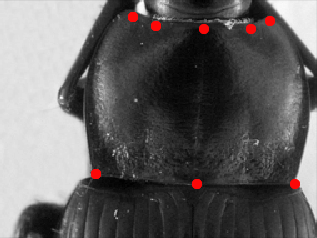
\includegraphics[height=1.2in]{images/fn_accuracy}
        \caption{\small{Image with well-predicted landmarks}}
        \label{figsub1}
    \end{subfigure}%
    ~ 
    \begin{subfigure}[t]{0.25\textwidth}
        \centering
        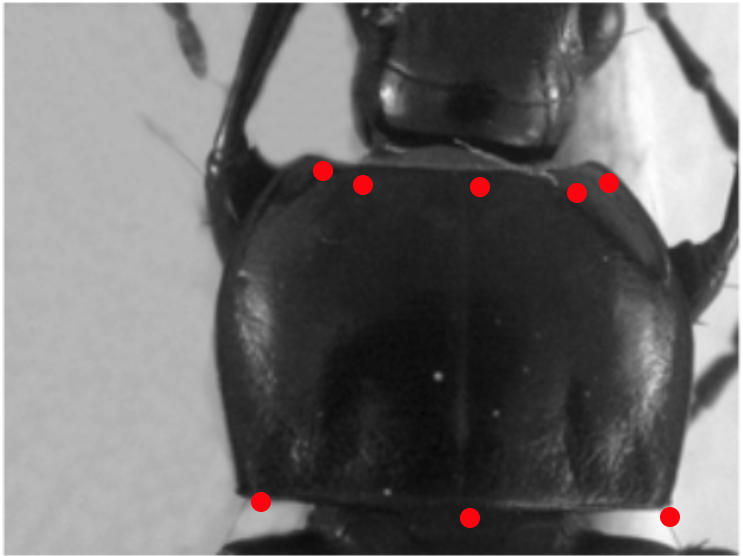
\includegraphics[height=1.2in]{images/plandmark2}
        \caption{\small{Image with inaccuracy landmarks}}
        \label{figsub2}
    \end{subfigure}
    \caption{\small{The predicted landmarks, in red,  on the images in test set.}}
    \label{figrsexample}
\end{figure}

\section{Fine-tuning to transfer learning}
\label{secimproving}
In section \ref{sectrain1}, the proposed network has been experimented
by training from scratch on pronotum dataset. The results of
experiments have shown that the network has worked well to detect the
landmarks on the pronotum images. However, when we consider the
predicted landmarks by displaying the landmarks on the images, the
result is still not precise, the average error still high ($\geq 4$
pixels).


In order to reach more acceptable results for biologists, we have
broadened the model with the step of transfer learning. That is a
method that re-uses the model developed for a specific task/dataset
to lead  another task with another dataset. This allows rapid progress or improved the performance of the
model on the second task \cite{torrey2009transfer}. The most popular
example has been given with the project ImageNet of Google \cite{put
  the ref} which has labelled several millions of images. The obtained parameter values can
be used in another context to classify another dataset, eventually
very different dataset \cite{put ref on MRI images}. The name of this procedure to re-use parameters
to pre-train a model is called \textit{fine-tuning}.

Fine-tuning is not only to replace and to retrain the model on the new
dataset, but also to fine-tune the weight of trained model by continuing the
backpropagation. Unfortunatly some rapid tests have shown that
re-using ImageNet features has not been relevant for our
application. We have designed a way to reproduce the method with our
own data, of course the size of the used data has been drastically decreased.
In that way, the network has been trained on a dataset including
the images of three parts of beetle i.e pronotum, body and head. Then,
the trained model will be used to fine-tune and test on pronotum set.


\subsection{Training data preparation}
The training dataset includes a combination of the images from three
sets: pronotum, body and head (Fig.\ref{figshape3parts}). For each
set, $260$ original images have been chosen radomly for training and
validation. By applying the same procedure in section \ref{sec_data},
the training dataset was enlarged to $5460$ images ($260 \times 7
\times 3$). However, the number of manual landmarks on each part is
difference: \textit{$8$ landmarks on pronotum part, $11$ landmarks on
  body part, and $10$ landmarks on head part}. The manual landmarks
have a specific meaning for the biologists. So, we can not insert the
landmarks arbitrarily. Instead of, we will keep the smallest number of
landmarks among three parts and we remove some landmarks on other
parts. Therefore, we kept the number of the landmark on pronotum as a
reference and we suppressed some landmarks on the body and head
part. Specifically, we have removed three landmarks on the body part
($1^{st}; 6^{t}h; 9^{th}$) and two landmarks on the head part ($5{th};
6^{th}$) (Fig.\ref{figshape3parts}).


\begin{figure}[htbp]

        \centering
        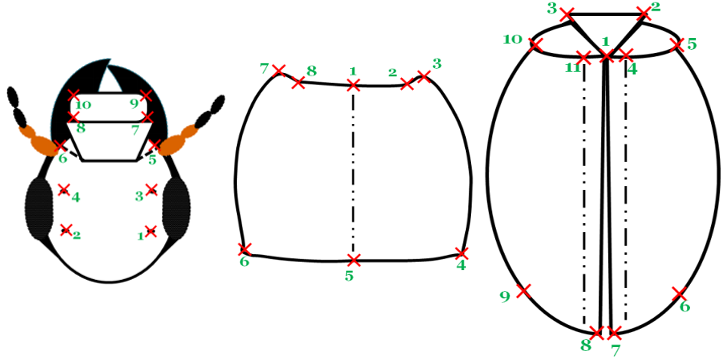
\includegraphics[scale=0.25]{images/merge}
 
 
    \caption{\small{A presentation of head, pronotum and body part with corresponding manual landmarks}} 
    \label{figshape3parts}
\end{figure}

\subsection{Using fine-tuning for pronotum dataset}

At the first step, the network is trained with $5460$ images following
the same way than explained in (section \ref{secmodel}). After that, 
this trained model has used to fine-tune the pronotum dataset. To compare the result with
the previous one, the trained model has been fine-tuned in many rounds
with different datasets. The losses during fine-tuning are shown in
Table.\ref{tblfinetuningloss}. Comparing with the losses when we
trained the model from scratch (Table. \ref{tbltrainingloss}), the
validation losses of this scenario have been significantly improved (around
$40\%$).

\begin{table}[h!]
	\centering
	\begin{tabular}{l l l}
	Round & Training loss & Validation loss \\ \hline
	1 & 0.00019 & 0.00009  \\ \hline
	2 & 0.00018 & 0.00010 \\ \hline
	3 & 0.00018 & 0.00010 \\ \hline
	4 & 0.00019 & 0.00008 \\ \hline
	5 & 0.00019 & 0.00009 \\ \hline
	6 & 0.00018 & 0.00008 \\ \hline
	7 & 0.00019 & 0.00008 \\ \hline
	8 & 0.00018 & 0.00006 \\ \hline
	9 & 0.00018 & 0.00009 \\ \hline
	\end{tabular}
	\caption{The losses during fine-tuning model}
	\label{tblfinetuningloss}
\end{table}

The output model has been used to predict the landmarks on the test
images. Then, average error based on the distance between
predicted and corresponding manual landmarks has been computed. The results
are shown in Table.\ref{tab2}. The \textbf{Distance 1} column reminds
the average distance obtained previously. The \textbf{Distance 2}
column presents for the new average distance
after fine-tuning the pronotum from the trained model. The
\textbf{Percentage} column contains the ratio of improvements. It is
clearly shown that the result of predicted landmarks with the help of
fine-tuning is more precise than the first way to do it.



\begin{table}[htbp]
\centering
\begin{tabular}{ | c | c | c | c | c | }
\hline
	\multicolumn{1}{|c|}{\multirow{2}{*}{Landmark}} & \multicolumn{2}{c|}{CNN} &  \multicolumn{2}{c|}{Fine-tuning}  \\ \cline{2-5}
	 & Average & SD & Average & SD \  \\ \hline
	\textbf{LM1} & \textbf{4.002} & \textbf{2.5732} & \textbf{2.486} & \textbf{1.5448} \\ \hline
	LM2 & 4.4831 & 2.7583 & 2.7198 & 1.7822 \\ \hline
	LM3 & 4.2959 & 2.7067 & 2.6523 & 1.8386 \\ \hline
	LM4 & 4.3865 & 3.0563 & 2.7709 & 1.9483 \\ \hline
	LM5 & 4.2925 & 2.9086 & 2.4872 & 1.6235 \\ \hline
	\textbf{LM6} & \textbf{5.3631} & \textbf{3.4234} & \textbf{3.0492} & \textbf{1.991} \\ \hline
	LM7 & 4.636 & 2.8426 & 2.6836 & 1.7781 \\ \hline
	LM8 & 4.9363 & 3.0801 & 2.8709 & 1.9662 \\ \hline
\end{tabular}
\caption{A comparing between the average error distances, the standard deviation values per landmark of two steps.}
\label{tab2}
\end{table}
To illustrate the final results, we display the distribution fo the
distance of both the best and the worst results (resp. landamark $1$
and $6$). The Fig.\ref{figrsexample2} shown in (a) and (b) diagrams
 how much the average distance and standard error (red lines) have
 been improved for the landmark $1$, the (c) and (d) diagrams for the
 landmark $6$.
\begin{figure}[htbp]
   
    \begin{subfigure}[t]{0.25\textwidth}
        \centering
        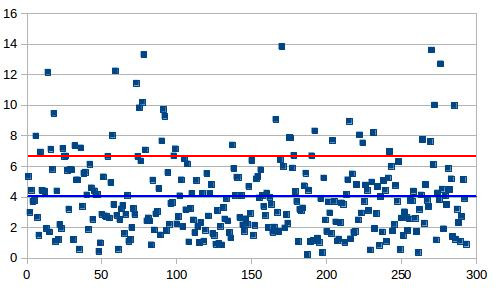
\includegraphics[scale=.35]{images/lm1_cnn_2}
        \caption{\small{Landmark 1 - CNN}}
        \label{figsub11}
    \end{subfigure}%
    ~ 
    \begin{subfigure}[t]{0.25\textwidth}
        \centering
        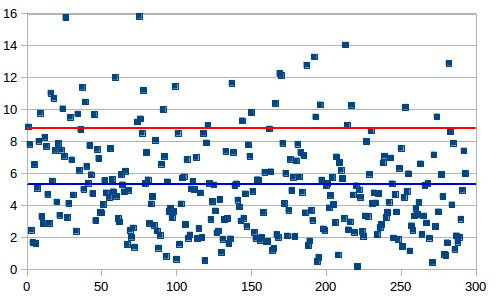
\includegraphics[scale=.34]{images/lm6_cnn_2}
        \caption{\small{Landmark 6 - CNN}}
        \label{figsub22}
    \end{subfigure}~\\
    \begin{subfigure}[t]{0.25\textwidth}
        \centering
        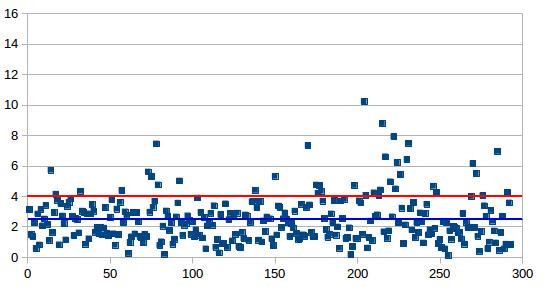
\includegraphics[scale=.33]{images/lm1_finetuning_2}
        \caption{\small{Landmark 1 - fine-tuning}}
        \label{figsub111}
    \end{subfigure}%
    ~ 
    \begin{subfigure}[t]{0.25\textwidth}
        \centering
        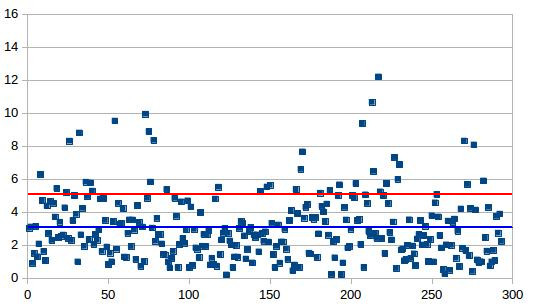
\includegraphics[scale=.32]{images/lm6_finetuning_2}
        \caption{\small{Landmark 6 - fine-tuning}}
        \label{figsub222}
    \end{subfigure}
    \caption{\small{The distribution of distance error on $1^{st}$ and $6^{th}$ landmarks of all images in two testing step(CNN and fine-tuning). The blue and red lines present for the average distances and standard deviation values, respectively.}}
    \label{figrsexample2}
\end{figure}

\section{Conclusion}
In this paper, we have presented a CNN with two scenarios to predict the landmarks on beetle's pronotum images. The CNN network has been designed with three times repeated structure which consists of a convolutional layer, a max pooling layer, and a dropout layer, followed by the connected layers. In the training phase, the CNN have been trained with several times in different selections of training data. After training, the network was able to predict the landmarks on the images in the test set. 

In the first scenario, the model has been trained (from scratch) and tested on the dataset of pronotum images. While in the second scenario, the model has been trained on a dataset includes the images from three parts of beetles. Then, the trained model has been used to fine-tune and test on pronotum images.

The result has been evaluated by comparing the coordinates between predicted and manual landmarks.  The results have shown that using the convolutional network to predict the landmarks on biological images is promising good results in the case that the image was difficult to segment. The quality of prediction allows using automatic landmarking to replace manual landmarks in some aspects. Training model from scratch or fine-tuning the trained model are given the acceptable results. But with a limited number of data, we need to improve the results a little bit. Therefore, future research in landmarking identification appears as an improved of the worth exploring.

\section*{Acknowledgements}
The research has been supported by DevMap project. We would like to thank the my colleague, ALEXIA Marie, who have provided manual landmarks on beetle images.

\bibliography{IEEEabrv,includes/icdp2009}


\end{document}






















the predicted landmarks by applying the second scenario on the same test images as Fig.\ref{figrsexample}. The red points present for the predicted landmarks. In Fig.\ref{figsub11}, the positions of predicted landmarks are the same when we compare with the result from Fig.\ref{figsub1}; but in Fig.\ref{figsub22}, the coordinates of predicted landmarks are strongly improved.
\begin{table}[htbp]
\centering
\begin{tabular}{|c|p{1.5cm}|}
\hline
\textbf{$\#$Landmark} & \textbf{Distance} \\ \hline
1 & 4.002  \\ \hline
2 & 4.4831 \\ \hline
3 & 4.2959 \\ \hline
4 & 4.3865 \\ \hline
5 & 4.2925 \\ \hline
6 & 5.3631 \\ \hline
7 & 4.636 \\ \hline
8 & 4.9363 \\ \hline
\end{tabular}
\caption{The average error distance per landmark}
\label{tabledistance}
\end{table}

\begin{table}[htbp]
\begin{center}
\begin{tabular}{|c|c|c|c|}
\hline
\textbf{$\#$Landmark} & \textbf{Error 1} & \textbf{Error 2} & \textbf{Improved($\%$)} \\ \hline
\textbf{1} & \textbf{4.002} & \textbf{2.486} & \textbf{37.88} \\ \hline
2 & 4.4831 & 2.720 & 39.33 \\ \hline
3 & 4.2959  & 2.652 & 38.27 \\ \hline
4 & 4.3865  & 2.771 & 36.83 \\ \hline
5 & 4.2925  & 2.487 & 42.06 \\ \hline
\textbf{6} & \textbf{5.3631}  & \textbf{3.049} & \textbf{43.15} \\ \hline
7 & 4.636  & 2.684 & 42.11 \\ \hline
8 & 4.9363  & 2.871 & 41.84 \\ \hline
\end{tabular}
\caption{The average error distance per landmark.}
\label{tab2}
\end{center}
\end{table}
